\documentclass[a4paper]{article}
\usepackage{amsfonts}
\usepackage{amsmath}
\usepackage{amssymb}
\usepackage{graphicx}     
\newcommand{\ddx}{\dfrac{d}{dx}}
\newcommand{\ddg}{\dfrac{d}{dg}}
\newcommand{\dint}{\displaystyle\int}

\begin{document}
  
\noindent \large Auteur: Luca Letroye \\
\noindent \large Studierichting: Informatica\\
\noindent \large Oefeningenreeks 5G nr. 3.1

\medskip
\normalsize

$f(x) = e^{-x} $ op $[0,+\infty[$\\

$V = \pi \lim\limits_{t\rightarrow+\infty} \dint_0^t e^{-2x}dx $\\

$= \pi \lim\limits_{t\rightarrow+\infty} \left[ \dfrac{-1}{2}e^{-2x}\right]_0^t$\\

$ = \pi \lim\limits_{t\rightarrow+\infty} \left(\dfrac{-e^{-2x}}{2}+\dfrac{1}{2}\right) = \dfrac{\pi}{2}$\\




\begin{figure}[h]
    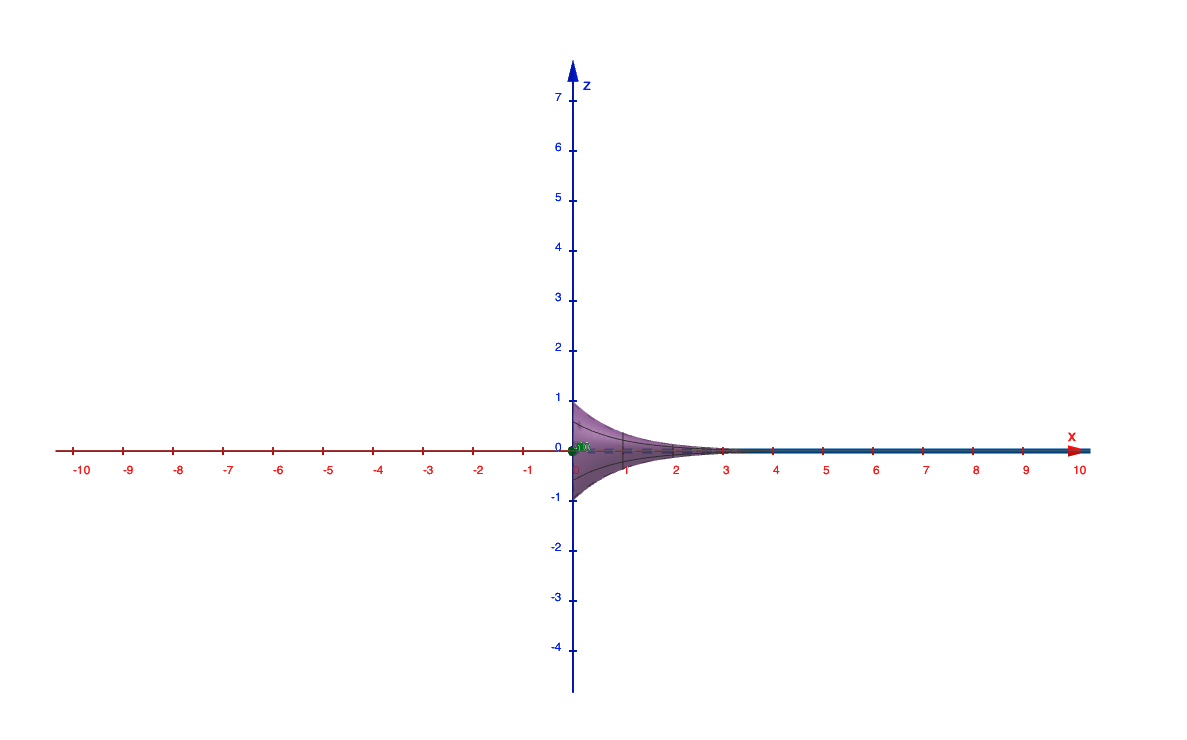
\includegraphics[width=\linewidth]{5G-3.1-luca.letroye.INF.png}\\
\end{figure}



\begin{thebibliography}{999}
%\bibitem{a} Referentie
\end{thebibliography}
\end{document} 
